\documentclass{article}
\usepackage[T1]{fontenc}
\usepackage[utf8]{inputenc}
\usepackage[lbd,submission]{ismir}
\usepackage{amsmath,cite,url}
\usepackage{graphicx}
\usepackage{color}
\usepackage{booktabs}
\usepackage{microtype}
\def\lbd{}

\setlength{\floatsep}{20pt plus 3pt minus 2pt}

\title{Can Notes Alone Be Jazzy?}

\oneauthor
 {Robert Wienroeder}
 {Berliner Hochschule f\"ur Technik, Cognitive Algorithms Lab \\ {\tt kontakt@robert-wienroeder.de}}

\def\authorname{R. Wienroeder}

\sloppy

\begin{document}

\maketitle

\begin{abstract}
What is jazz? Most people would say it is improvisation, it lives in the moment, 
and it cannot be fully captured
on paper. This study asks if there is still anything about jazziness that a model 
can learn, and that listeners are also able to distinguish.
For that purpose, a melodic Variational Autoencoder (VAE) is trained on 4-bar 
melody tokens from classical music and jazz melody datasets.
From this latent space, a jazz axis is extracted that can be used
to increase or decrease the ``jazziness'' of a melody.
A first model gave high separability (AUC 0.99) but was reading input format rather than genre; 
to remove this shortcut, we balance both formats for both genres in the training data.
The resulting axis shows only slightly lower separability
(AUC 0.89) while putting jazz samples reliably on the jazz side, no matter if the 
source is lead sheets or live performances.
We find that the axis tracks syncopation and chromaticism
rather than note density.
In a blind and order-randomised pilot, the author, a professional 
jazz musician, identified the jazzier of two steered versions of the same 
melody in 17 of 18 cases;
a larger listening study is in preparation.
\end{abstract}

\section{Introduction}\label{sec:introduction}

VAEs over symbolic music are well established~\cite{roberts2018musicvae}.
Jiang et al.~\cite{jiang2025composervector} find axes based on composer style, while we try
to find axes based on genre.
Pati and Lerch~\cite{pati2021attribute} regularise attributes onto single latent 
dimensions during training. We follow a different approach and construct the axis
after training from the learned vector space. A style axis can show very high separability but read
something different from style. Musical datasets usually contain data of a specific genre,
so certain dataset properties (like transcriptions vs. scores) could get modelled rather 
than the actual style of a melody.
Therefore, the test datasets cover both genres in both formats.


\section{Data and Model}\label{sec:data}

\textbf{Real beats.} Tokens are notes (rest, hold or onset of one of 128 
possible pitches) on a 16th note grid with 4 bars or 64 steps per window,
so one musical piece can provide several windows. We cap at 64 windows per piece
to not let an individual piece over-influence the model.
Beat positions come from annotated beats for the performance corpora and from
notation for the scores and never from a fixed tempo, which would push
almost every live performance off the grid 
and make it seem syncopated where it is not.
\\Jazz datasets:
\begin{itemize}\setlength{\itemsep}{0pt}\setlength{\parskip}{0pt}
\item Weimar Jazz Database (WJazzD): jazz solos~\cite{pfleiderer2017jazzomat}
\item PDMX: jazz-tagged scores, one melodic track~\cite{long2025pdmx}
\item Jazz Trio Database: piano transcriptions~\cite{cheston2024jtd}
\end{itemize}
Classical datasets:
\begin{itemize}\setlength{\itemsep}{0pt}\setlength{\parskip}{0pt}
\item OpenScore Lieder: vocal lines from the score~\cite{gotham2018scores}
\item ASAP: classical piano performances~\cite{foscarin2020asap}
\item OpenScore string quartets: first violin~\cite{openscorequartets}
\end{itemize}
Only passages in 4/4, 2/4 and 2/2 are kept. For piano performances the top voice 
is being used, and only samples with a mean interval of less than 5 semitones 
and a maximum of 10\% intervals greater than a fifth, to avoid using just the top note
of piano accompaniment as melodies. Every piece is
transposed to C and shifted to a median pitch within an octave of G4, so that key and register cannot be used 
as proxies for the genre separation. Keys are estimated with the Krumhansl-Schmuckler
algorithm~\cite{krumhansl1990pitch} using the Krumhansl-Kessler
profiles~\cite{krumhansl1982keys}, per piece. After this normalisation the per-window tonic
distributions of the two genres are near-identical (total variation distance
0.062).

\textbf{Balanced training.} Each genre gets both formats in equal amounts:
jazz gets PDMX for scores and JTD for performance, classical gets Lieder for scores and ASAP 
for performance, 1,996 windows per cell. JTD is split by pianist and ASAP by
composer to ensure the model cannot just learn a certain pianist or composer style; 
30\% of each, plus all of the quartets and all of WJazzD are held out.

\textbf{Model and axis.} The model consists of an encoder that is a bidirectional GRU 
with 512 per direction, and a decoder GRU with 512 units. The latent space consists of 128 dimensions.
All windows are randomly transposed by up to 3 semitones in either direction during training. 
The ``jazz axis'' the model is reading is the vector from the centroid of the classical melody embeddings
to the centroid of the jazz melody embeddings. To fit the axis all four dataset types
(classical and jazz, performance and scores) are re-sampled to only windows with matching note counts
to make sure note count cannot define the axis.

\section{Results}\label{sec:results}

\textbf{Held-out test.} We project each holdout dataset's windows onto the jazz
axis and measure the AUC metric against the in-sample classical and the in-sample
jazz embeddings (\tabref{tab:heldout}).
The first model confounded genre and format and modelled performance vs. written score
rather than jazz vs. classical, and thus classified classical performances as jazz (\figref{fig:confound}). 
After balancing both formats in both genres in the training data, all jazz test sets
land on the jazz side, regardless of data format.
\tabref{tab:heldout} shows that the model still performs weakly on ASAP. Here, 
unseen composers fall between the jazz and the classical cluster, likely
because dense piano runs have a lot of offbeats
involved on a 16th note grid (where 3/4 of notes in a continuous 16th note run are classified as off-beats). 
PDMX Jazz is also still clearly sitting below jazz on the axis: 
the reason might be that this dataset is not very strict and contains ragtime and pop, too.
In-sample separability between jazz and classical is 0.89, and the axis correlates
with syncopation ($r=0.48$, measured with the Longuet-Higgins and Lee
syncopation measure~\cite{longuethiggins1984rhythmic}) and chromaticism
($0.28$), but not with density ($0.06$).

\textbf{Descriptor baselines.} A high separability could theoretically also be
achieved without a learned vector space. So we try to separate the genres using
a descriptor instead of the embeddings. Syncopation~\cite{longuethiggins1984rhythmic} 
places all five test sets in the correct genre region and separates the genres
with an AUC of 0.855. The axis reaches 0.894 and also tracks several descriptors at once, 
but the difference in AUC is genuinely small. The separability should therefore be used
to validate the axis, but not as its main result. A descriptor like syncopation can classify a melody, 
but it can not move the melody along an axis and decode the latent space into a new melody, like the VAE can.

\begin{figure}[!t]
 \centering
 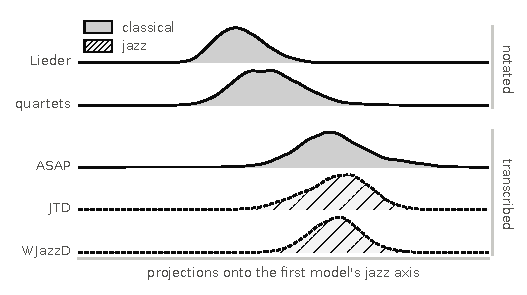
\includegraphics[width=\columnwidth]{fig_confound.pdf}
 \caption{What the first model learned. The projections are clearly grouped together
 by format and not by genre. The three transcribed performance datasets are aligned
 together, which means classical ASAP is grouped together with the jazz
 solos.}
 \label{fig:confound}
\end{figure}

\begin{table}[!t]
 \centering
 \footnotesize
 \setlength{\tabcolsep}{4pt}
 \begin{tabular}{llrcc}
  \toprule
  held-out & genre, format & $n$ & vs classical & vs jazz \\
  \midrule
  quartets & cl., sheet & 5,974 & \textbf{0.59} & 0.14 \\
  ASAP & cl., perf. & 1,562 & \textbf{0.81} & 0.30 \\
  JTD & jazz, perf. & 1,467 & 0.93 & \textbf{0.57} \\
  PDMX jazz & jazz, sheet & 2,270 & 0.78 & \textbf{0.33} \\
  WJazzD & jazz, solo & 12,748 & 0.94 & \textbf{0.60} \\
  \bottomrule
 \end{tabular}
 \caption{AUC of all test datasets' projections created by the final balanced model,
 against the in-sample classical and against the in-sample jazz samples. $n$ is the number of
 test windows. The two AUC columns are not comparable: \textbf{bold} shows each dataset's
 AUC value compared to samples of its own genre, which should optimally be close to 0.5.}
 \label{tab:heldout}
\end{table}

\textbf{Steering.} We conduct an experiment of steering 20 melodies that were included in the
training dataset from $-3$ to $+3$ standard
deviations along the axis. The decoder gets restricted to one octave around the original melody, 
and several samples are generated of which the one is kept that has the closest note count to the original.
Those 6 standard deviation steps along the axis raise syncopation from 0.53 to 0.71 and the
portion of out-of-scale notes from 2.2\% to 5.1\%. Note density does not move much (0.43 to 0.45).

\textbf{Blind pilot.} The author, a professional jazz musician, judged which of
two clips of the same melody that he had not heard before ($-3$ vs.\ $+3$, randomised order, 4-beat
count-in, 80~bpm, 2 bars) was jazzier. He chose the correct one in
17 of 18 cases (one-sided binomial $p=7\times10^{-5}$). Steering along the axis towards jazz tends to add
notes. Out of the 18 pairs, 5 had unequal note counts, and four out of those five had a jazzier sample
with \emph{fewer} notes. All five were judged correctly. Since the listener was the one who built the model, 
this is only a pilot of course.

\section{Discussion and Ongoing Work}\label{sec:discussion}

A melodic VAE can capture a component of jazziness that lives in the notes,
and an expert can hear it. Since the model is monophonic and samples live on a
straight 16th note MIDI grid, no harmony, swing feel, blue notes or articulation
can be considered. This is deliberate, since the goal was to find out if there is
jazziness in the notes alone and if it can be used to make melodies more or less
jazzy. Velocity was excluded because only
the performance datasets carry real dynamics, so it would just have been another proxy
for provenance rather than genre.
Using different input formats for all genres is relatively cheap and 
showed the data provenance shortcut the model was taking. We therefore recommend it for any
music genre axis. To improve AUC numbers for ASAP it could help to density-match 
the test sets during scoring and not only for the axis fit. 
A listening study with 20 participants
who did not build the model is in preparation.
A natural next step would be to extend this approach to other genres or polyphonic melodies and harmonies.
Another one would be to train the model so that the desired axis is represented by one latent dimension,
following the approach by Pati and Lerch~\cite{pati2021attribute}.

\section{AI Usage Statement}\label{sec:ai}

Large language models were used for research on related work and on potential datasets, to
outline the different project phases, and to summarise the experiments conducted in bullet point form
before writing the paper.
The author made every project and design decision himself, based on his experiences and knowledge,
verified every cited source, selected citations, and wrote all
text himself. The author takes full responsibility for all content, including the
correctness of all references and the correctness and originality of all text.

\bibliography{refs}

\end{document}
